\documentclass{beamer}

\usepackage{tikz}
\usepackage[utf8]{inputenc}
\usepackage{amsmath}
\usepackage{commath}
\usepackage{amssymb}
\usepackage{amsfonts}
\usepackage{epstopdf}
\usepackage{graphicx}
\usepackage{graphics}
\usepackage{listings}

\usetheme[CB,contents,colthm,colmath]{Mittweida}

\author{Felix Haller, Konstantin Lorenz}
\title{REST Beleg}
\subtitle{Projektverwaltung für Studenten und Professoren}
\institute{IF13wI-B}
\date{}

\begin{document}

	\maketitle

	\nextframenocontents

	\section*{Inhalt}
	\begin{frame}{Inhalt}
		\tableofcontents
	\end{frame}
	\section{Aufgabenstellung}
		\begin{frame}{Aufgabenstellung}
			\begin{itemize}
				\item lauffähiger RESTful Webservice
				\item Testclient
				\item technische Dokumentation
			\end{itemize}
		\end{frame}
		
	\section{Motivation}
		\begin{frame}{Motivation}
			\begin{itemize}
				\item Anlaufstelle zur Bekanntmachung von Projekten
				\item Vernetzung während Planung/Durchführung
				\item Studenten
				\begin{itemize}
					\item Finden geeigneter Projekte für 
					\begin{itemize}
						\item Belege
						\item Abschlussarbeiten
					\end{itemize}
					\item Vertiefen von Interessen	
				\end{itemize}
				\item Professoren
				\begin{itemize}
					\item Forschungsgruppen/-arbeiten
					\item Hochschulprojekte (z.B. HSMWmobil)
				\end{itemize}
			\end{itemize}
		\end{frame}
		
	\section{Bedienkonzept}
		\begin{frame}{Bedienkonzept - Methoden}
			\begin{itemize}
				\item GET - Objekte abrufen
				\begin{itemize}
					\item Ressourcenaufruf per URI (Pfad Parameter)
					\item Filterung durch \textbf{Query} Parameter
				\end{itemize}
				\item POST - Objekt erstellen
					\begin{itemize}
						\item Auswahl des Ortes per URI (Pfad Parameter)
						\item Attribute über \textbf{Form} Parameter 
					\end{itemize}
				\item PUT - Objekte bearbeiten
					\begin{itemize}
						\item Auswahl der Ressource per URI (Pfad Parameter)
						\item geänderte Attribute über \textbf{Form} Parameter 
					\end{itemize}
				\item DELETE - Objekte löschen	
				\begin{itemize}
					\item Auswahl der Ressource per URI (Pfad Parameter) 
				\end{itemize}
			\end{itemize}
		\end{frame}
		
		\begin{frame}{Bedienkonzept - Aufrufe}
			\begin{block}{statische Ressourcen}
				\begin{itemize}
					\item URI führt zu eindeutiger Ressource
					\item z.B.: Projekt mit ID 1: \textbf{/projects/1}
				\end{itemize}
			\end{block}	
			
			\begin{block}{Ressourcen Sammlungen}
				\begin{itemize}
					\item URI führt zu Sammlung von Ressourcen
					\item z.B.: alle Projekte \textbf{/projects}
					\item durch Query Parameter filterbar
					\item z.B.: alle Projekte von tutnix:\\
					\textbf{/projects/?creator=tutnix}
				\end{itemize}
			\end{block}	
			
		\end{frame}
	\section{Übersicht REST Ressourcen}
		\begin{frame}{Übersicht REST Ressourcen}
			\begin{figure}
				\centering
				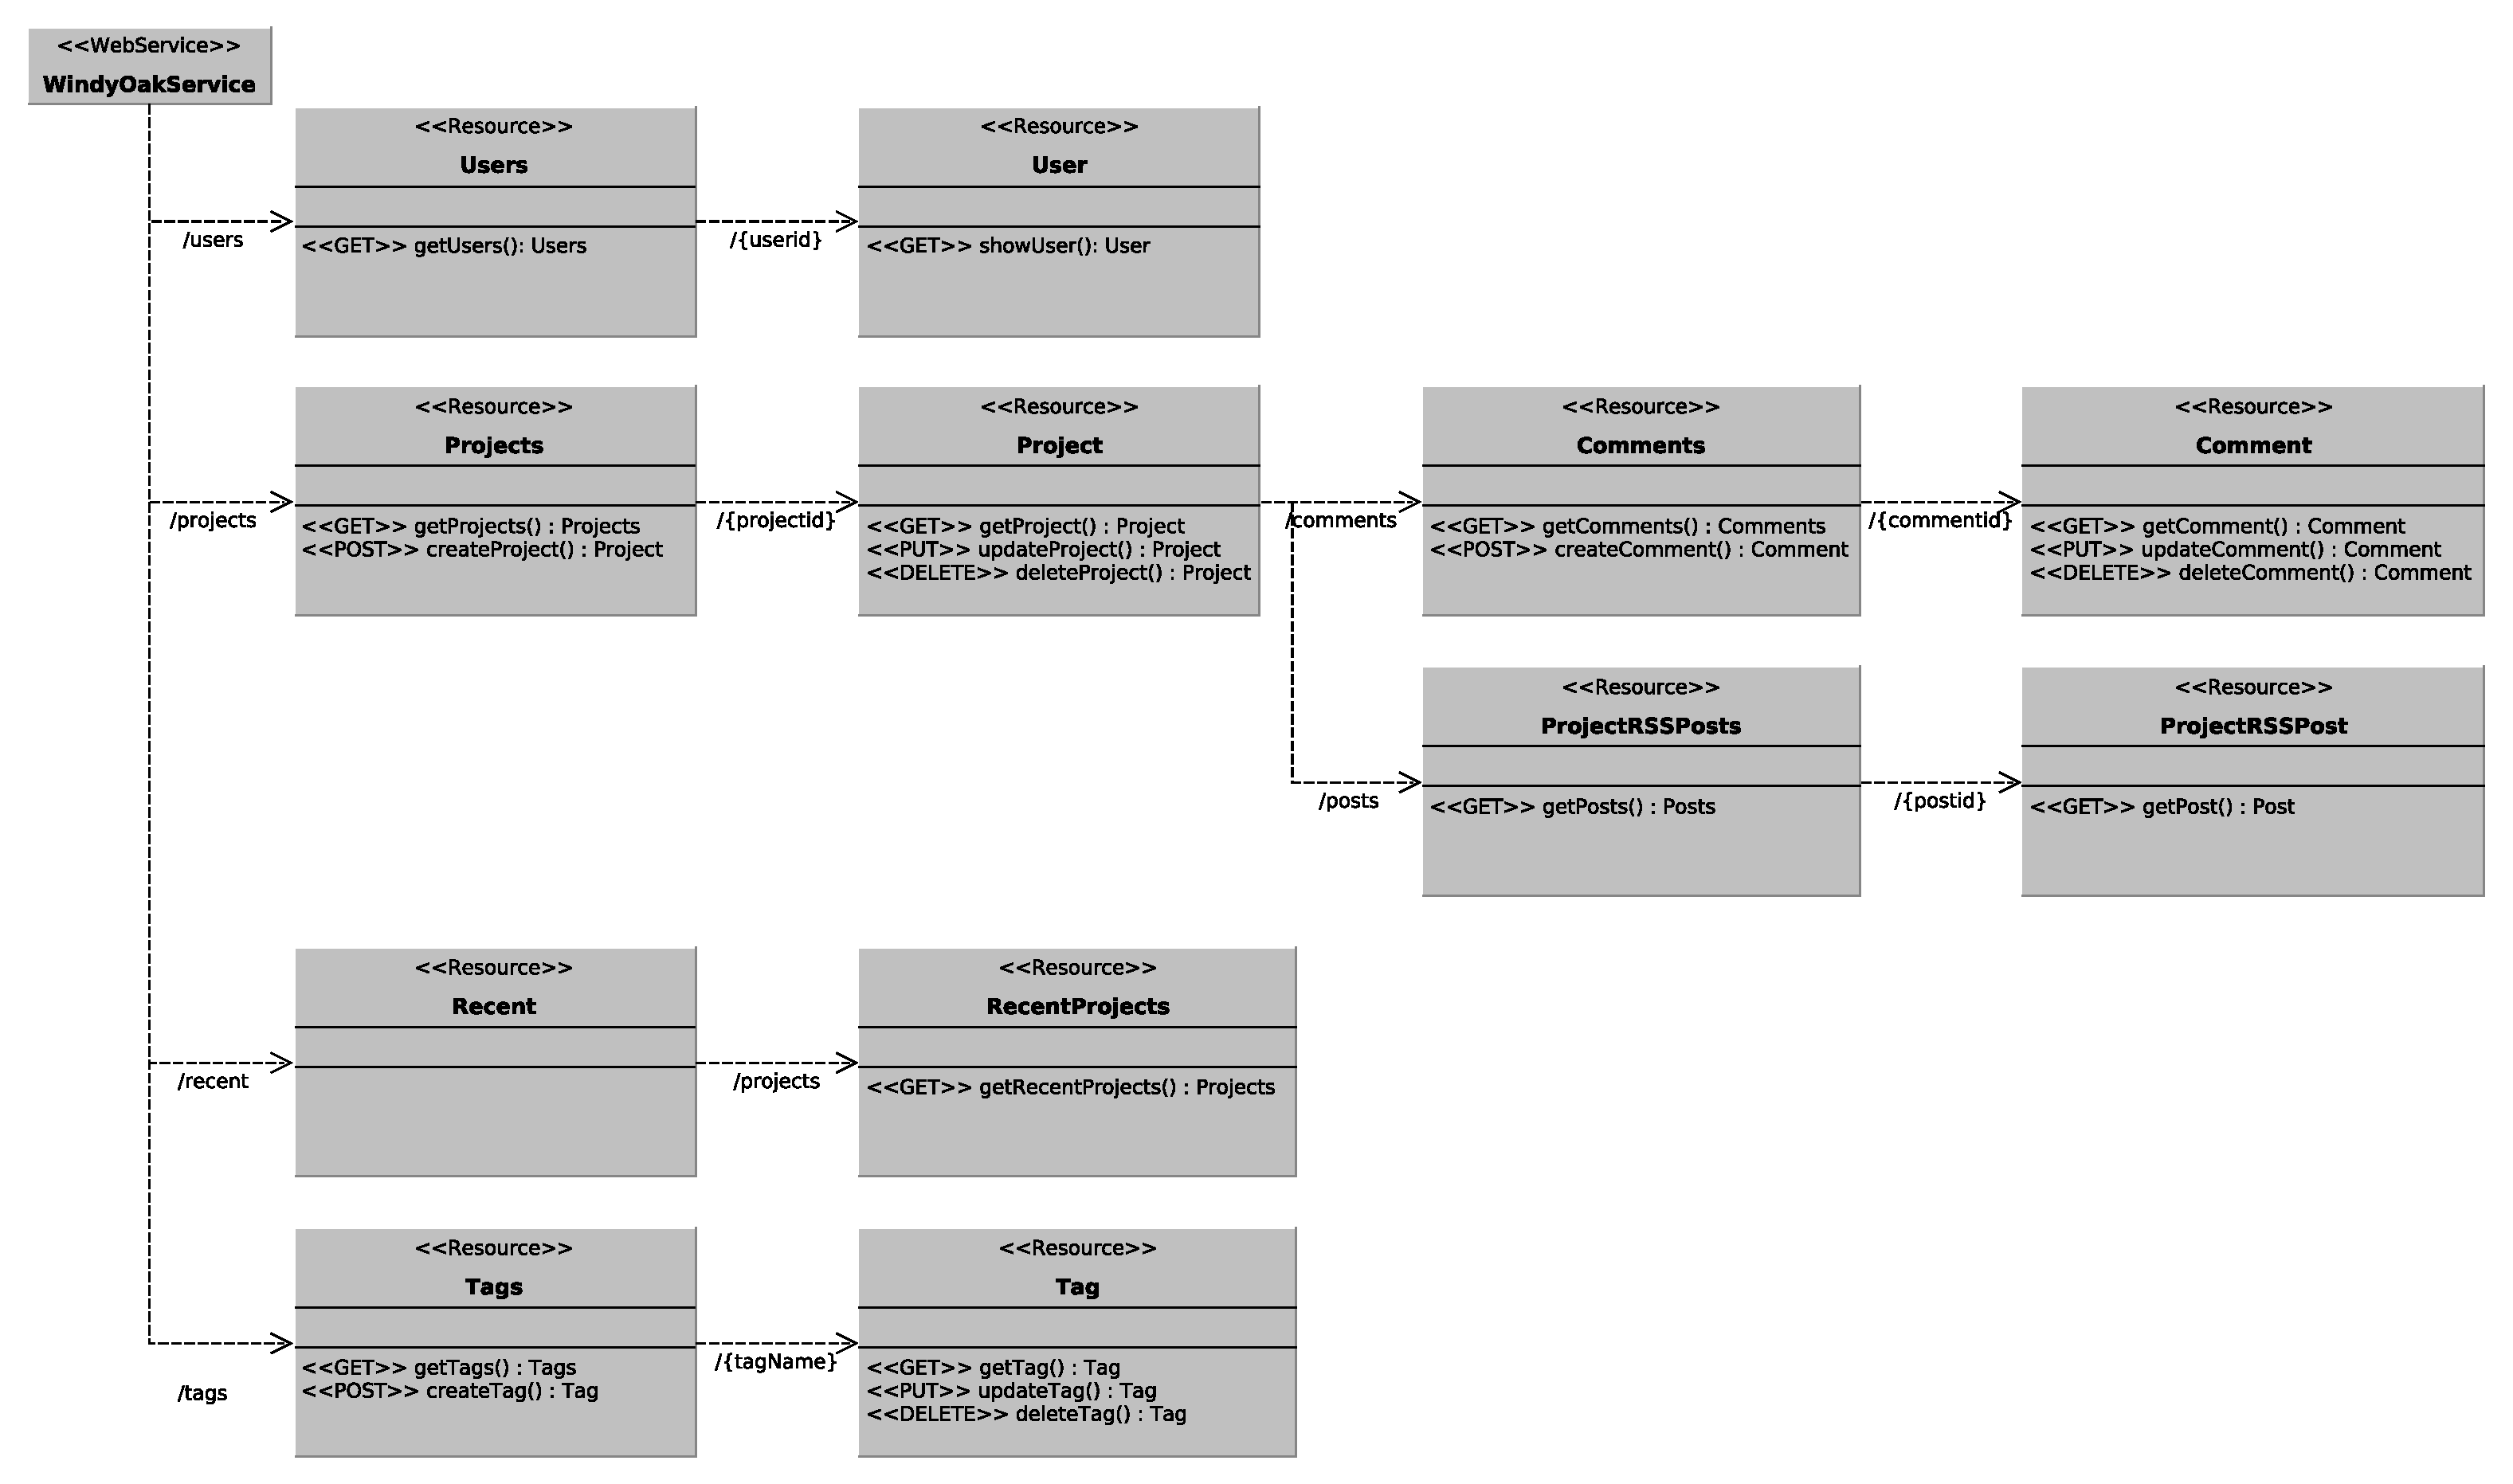
\includegraphics[width=1.05\linewidth]{Bilder/rest.pdf}
			\end{figure}
		\end{frame}
	\section{Testszenario}
		\begin{frame}{Testszenario}
			\begin{itemize}
				\item Demonstration der Funktionalität
				\item Client zeigt Rückgabe als XML
				\item Ausgabe von Statuscodes
				\item Führung des Anwenders
			\end{itemize}
			\begin{block}{Anwendungsszenarien:}
				\begin{itemize}
					\item Projekte
					\item Kommentare
					\item Tags
					\item RSS-Posts
				\end{itemize}
			\end{block}
		\end{frame}
		\begin{frame}{Client Demo}
			Client Demo...
		\end{frame}
	\section{Live Aufrufe von einigen REST Befehlen}
		\begin{frame}{Live REST Abfragen}
			Live Demo...
		\end{frame}
\end{document}